\section{Рекурсивные вычисления}
\subsection{Условие задания}
Выполнить задание. Номер варианта --- 4.

Создать рекурсивную функцию, вычисляющую значение полинома Эрмита:
\begin{equation}
\begin{cases}
     H_0(x) = 1,\\
     H_1(x) = 2x,\\
     H_n(x) = 2x \times H_{n-1}(x) - 2n \times H_{n-2}(x).\\
\end{cases}
\end{equation}

Проверить работу созданного приложения на приведённых тестовых примерах. 

Приложение должно содержать следующие компоненты:
\begin{enumerate}
\item Заголовок формы должен отражать суть задания.
\item Все элементы формы должны быть внятно подписаны (кнопки подписаны, у тестового поля должно быть написано, для чего оно нужно и т. д.)
\item В коде должны быть комментарии и отступы (код должен быть легко читаем).
\item В коде программы все элементы формы должны быть переименованы (btnName -  для кнопок, lblName - для ссылок, txtName - для текстового поля и т. д.) Наименования должны быть понятными.
\item Приложение должно корректно работать (выводить ответ или ошибку с соответствующим сообщением) для следующих данных: ввод буквы, ввод отрицательного числа, ввод нуля, ввод положительного числа (< 10), ввод большого положительного числа. После вывода ошибок при вводе корректных данных поля ошибок должны очищаться.
\end{enumerate}

\subsection{Вид формы в конструкторе}
Форма имеет вид:

\begin{figure}
\centering
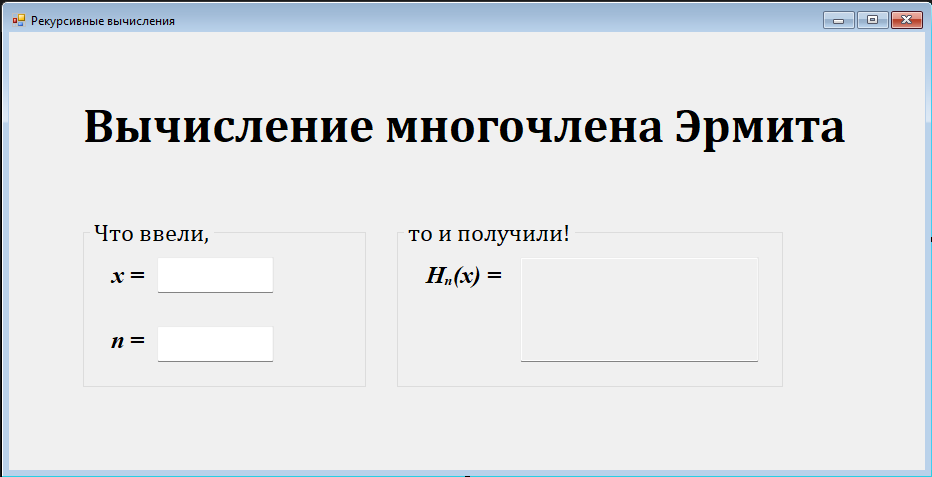
\includegraphics[width=0.5\linewidth]{images/recursive-calculations/form.png}
\caption{Форма окна для задания <<Рекурсивные вычисления>>}
\label{recursive-calculations-form}
\end{figure}

\subsection{Таблица с описанием элементов формы}
Все элементы формы были переименованы для большей читаемости. В таблице \ref{tab:recursive-calculations-form} представлены все изменения.

\begin{table}
\centering
\begin{tabular}{|m{0.3\textwidth}|m{0.3\textwidth}|m{0.3\textwidth}|}
\hline
\textbf{Описание элементов формы} & \textbf{Список изменённых атрибутов} & \textbf{Новое значение атрибута} \\
\hline
\hline
Окно формы & Text & Рекурсивные вычисления \\
Заголовок & Name & mainTitle \\
Группа ввода & Name & inputGroup \\
Группа вывода & Name & outputGroup \\
Метка для X & Name & xLabel \\
Метка для N & Name & nLabel \\
Поле ввода для X & Name & xTextBox \\
Поле ввода для N & Name & nTextBox \\
Метка для значения многочлена & Name & outputLabel \\
Поле вывода для значения многочлена & Name & outputTextBox \\
\hline
\end{tabular}
\caption{Значение атрибутов элементов в приложении для рекурсивных вычислений}
\label{tab:recursive-calculations-form}
\end{table}

\subsection{Примеры правильной и неправильной работы приложения}
При запуске приложения на экране появляется окно \ref{fig:recursive-calculations-start}.

\begin{figure}
\centering
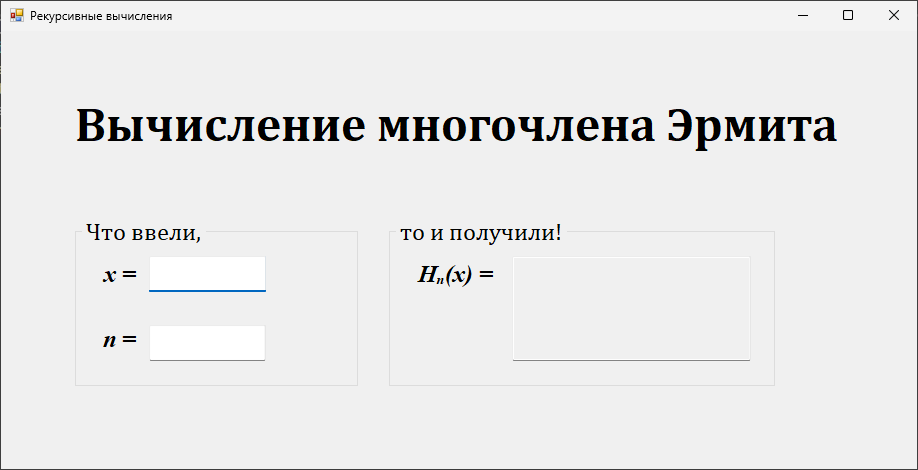
\includegraphics[width=0.5\linewidth]{images//recursive-calculations/start.png}
\caption{Запуск программы}
\label{fig:recursive-calculations-start}
\end{figure}

При изменении полей ввода реактивно подсчитывается и подставляется значение в поле вывода. Также происходит обработка ошибок.

\begin{figure}
\centering
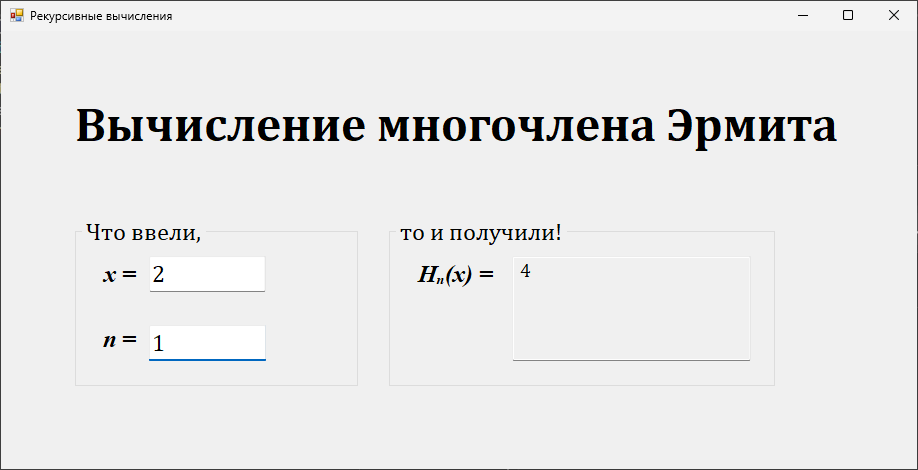
\includegraphics[width=0.5\linewidth]{images//recursive-calculations/okay.png}
\caption{Запуск с корректными данными}
\label{fig:recursive-calculations-okay}
\end{figure}

\begin{figure}
\centering
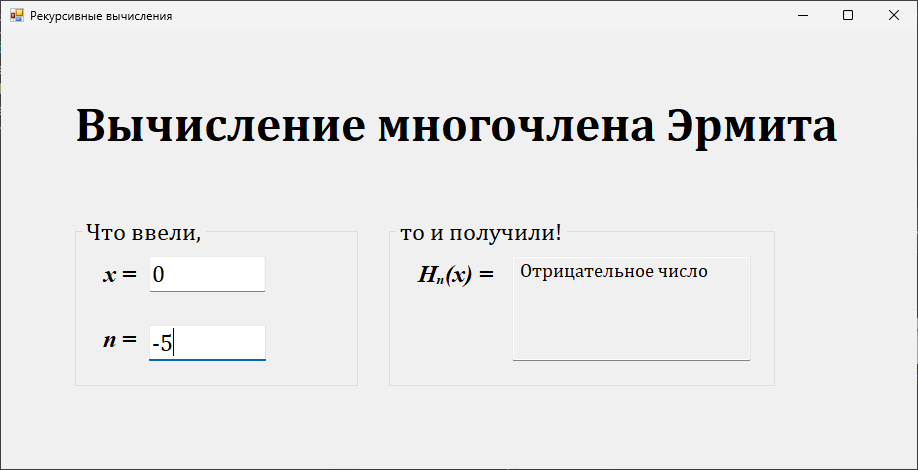
\includegraphics[width=0.5\linewidth]{images//recursive-calculations/error.png}
\caption{Пример ввода с некорректными данными}
\label{fig:recursive-calculations-error}
\end{figure}

\begin{figure}
\centering
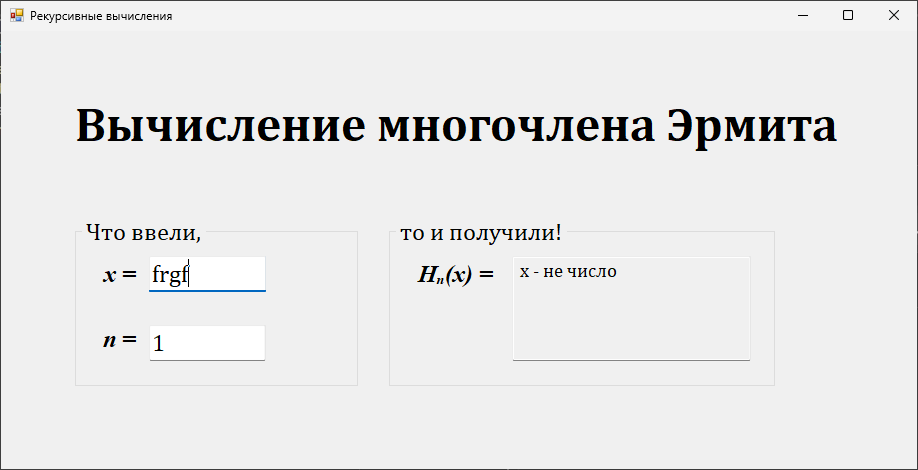
\includegraphics[width=0.5\linewidth]{images//recursive-calculations/error2.png}
\caption{Пример ввода с некорректными данными}
\label{fig:recursive-calculations-error2}
\end{figure}

\subsection{Примеры исходного кода}
\begin{minted}{cpp}
/* обработка события изменения полей */
private: System::Void recalculate(System::Object^ sender, System::EventArgs^ e) {
	double xInput = 0;
	bool resultX = Double::TryParse(this->xTextBox->Text, xInput);

	long long nInput = 0;
	bool resultN = Int64::TryParse(this->nTextBox->Text, nInput);

	if (!(resultX && resultN)) {
		if (resultN) {
			this->outputTextBox->Text = "x - не число";
		} else if (resultX) {
			this->outputTextBox->Text = "n - не целое число";
		} else {
			this->outputTextBox->Text = "x - не число, n - не целое число";
		}
	} else if (nInput < 0) {
		this->outputTextBox->Text = "Отрицательное число";
	}
	else {
		this->outputTextBox->Text = System::Convert::ToString(H(nInput, xInput));
	}
}
\end{minted}

Больше кода проекта доступно в приложении \ref{application-A}. Также в приложенном архиве можно найти полный код проекта.